\chapter{GPU-based Motion Planning} 
\label{chp:GPlanner}

\section{Introduction}
There is extensive literature on motion planning and global navigation. Practical methods for motion planning for high-DOF robots are often
based on randomized sampling~\cite{Kavraki96, Kuffner00}. These methods attempt to capture the topology of the free space
by generating random configurations and connecting nearby configurations using
local planning methods. The resulting algorithms are probabilistically complete and
have been successfully used to solve many high-DOF motion planning and
navigation problems in different applications. However, they are too slow for interactive applications or dynamic environments.


\subsection{Main Results}
We present a novel parallel algorithm
for real-time motion planning of high-DOF robots that exploits the computational capability of a \$400 commodity
graphics processing unit (GPU). Current GPUs are programmable many-core
processors that can support thousands of concurrent threads. We use
them for real-time computation of a probabilistic roadmap (PRM) and a lazy planner. We describe
efficient parallel strategies for constructing the roadmap that include
sample generation, collision detection, connecting nearby samples, and
local planning. The query phase is also performed in parallel based on graph search. In order to design an efficient single query planner, we use a lazy strategy that defers collision checking and local planning. We also describe new hierarchy-based collision detection algorithms, to accelerate the overall performance.

The performance of the algorithm is governed by the topology of the underlying
free space as well as the methods used for sample generation and nearest
neighbor computation. In practice, our algorithm can generate thousands of samples for
robots with 3 or 6 DOF and compute the roadmap for these samples at close to interactive rates, including construction of all hierarchies.
Our algorithm performs no precomputation and is applicable to dynamic scenes, articulated models, and non-rigid robots. We evaluate its
performance using multiple benchmarks on a commodity PC with a NVIDIA GTX 285 GPU and observe a 10 to 80-fold improvement in performance, compared to CPU-based implementations.

\subsection{Organization}
The rest of this chapter is organized as follows. We survey
related work on real-time motion planning and GPU-based algorithms in Section~\ref{sec:4:related}. Section~\ref{sec:4:overview} gives an overview of our approach and we present parallel algorithms for
the construction and query phase in Section~\ref{sec:4:algorithm}. We evaluate performance
on different motion planning benchmarks in Section~\ref{sec:4:result} and compare with prior
methods.

\section{Related Work}
\label{sec:4:related}
In this section, we first provide background on current GPU architectures. Next, we give a brief overview of prior work in real-time motion planning.

\subsection{GPU Architectures}
In recent years, the focus in processor
architectures has shifted from increasing clock rate to
increasing parallelism. Commodity GPUs such as NVIDIA Fermi
have theoretical peak performance of Tera-FLOP/s
for single precision
computations and hundreds of Giga-FLOP/s for double precision computations. This
peak performance is significantly higher than current multi-core CPUs, thus outpacing
CPU architectures~\cite{Lindholm2008} at relatively modest cost of \$400 to \$500.
However, GPUs have different architectural characteristics and a different memory hierarchy, which impose
constraints in terms of designing appropriate algorithms.
First, GPUs usually have a high number of independent cores (e.g., the newest generation GTX 480 has 15 cores and each core has
32 streaming processors, resulting in total of 480 processors while GTX 280 has 240 processors). Each of the individual cores
is a vector processor capable of performing the same operation
on several elements simultaneously (32 elements for
current GPUs). Second, the memory hierarchy on GPUs is quite different from that of CPUs, and cache sizes on GPUs are considerably smaller. Moreover, each GPU
core can handle several separate tasks in parallel and switch
between different tasks in the hardware when one of them is waiting for a
memory operation to complete. This hardware multi-threading
approach is designed to hide memory access latency. Third, all GPU threads are logically grouped in blocks with a per-block high-speed shared memory, which provides a weak synchronization capability between the GPU cores. Overall, shared memory is a limited resource on GPUs: increasing the shared memory distributed for each thread can limit the extent of parallelism. Finally, multiple GPU threads are physically managed and scheduled in
the \emph{single-instruction, multiple-thread} (SIMT) way, i.e., threads are grouped into chunks and each chunk executes one
common instruction at a time. In contrast to \emph{single-instruction multiple-data} (SIMD) schemes, the SIMT scheme allows each thread to have its own instruction address counter and register state, and therefore the freedom to branch and execute independently. However, a GPU's performance can reduce significantly when threads in the same chunk diverge considerably, because these diverging portions are executed in a serial manner for all the branches. As a result, threads with coherent branching decisions (e.g., threads traversing the same paths in the bounding volume hierarchy structure for two objects involving in collision checking) are preferred on GPUs in order to obtain higher performance~\cite{Gunther07}. All of these characteristics imply that -- unlike CPUs -- achieving high performance in current GPUs depends on several factors:
\begin{enumerate}
\item Generating a sufficient number of parallel tasks so that all the cores are highly utilized.
\item Developing parallel algorithms such that the total number of tasks is higher than the number of threads, so that each core has enough work to perform
while waiting for data from relatively slow memory accesses.
\item Assigning appropriate size for shared memory to accelerate memory accesses while not reducing the level of parallelism.
\item Performing coherent or similar branching decisions for each parallel thread within a given chunk.
\end{enumerate}
These requirements impose constraints in terms of designing appropriate collision query algorithms for running on GPUs.

\subsection{Real-time Motion Planning}
An excellent survey of various motion planning algorithms is given in~\cite{LaValle:2006}. Many parallel algorithms
have also been proposed for motion planning, that utilize the properties of configuration spaces~\cite{Perez91}.
The distributed representation of motion planning~\cite{BL91:rmp} can be easily parallelized. In order to deal with high dimensional
or difficult planning problems, distributed sampling-based techniques have been proposed~\cite{plaku+2007:OOPSM}.

The computational power of many-core GPUs has been used for many geometric
and scientific computations~\cite{GPGPU07}. The rasterization capabilities of
a GPU can be used for real-time motion planning of low DOF robots~\cite{Hoff00,Sud07} or for improving sample generation in narrow passages~\cite{PKLM00,FGLM01}.

\section{Overview}
\label{sec:4:overview}
In this section, we discuss some challenges in developing parallel motion planning algorithms for current GPU architectures. One of our goals is to use sample-based planners that are relatively easy to parallelize and can be used for single query and multiple queries.

We choose the PRM algorithm as the underlying method for parallel planning, because it is most suitable to exploit multiple cores and data parallelism on GPUs. The PRM algorithm is composed of several steps and each step performs similar operations on the input samples or the links joining those samples. Many other efficient CPU-based algorithms have also been developed, including RRT~\cite{Kuffner00} and SBL~\cite{SL01}. However, these methods may not be able to exploit the GPU parallelism due to two reasons. First, these methods proceed in an incremental manner in terms of adding new samples to the underlying tree structure. Second, the order of adding new samples is critical in determining the expansion of the tree.

The PRM algorithm has two phases: roadmap construction and querying. The roadmap construction phase includes four main steps: 1) generate samples in the configuration space; 2) compute milestones that correspond to the samples in the free space by performing discrete collision queries; 3) for each milestone, find other milestones that are nearest to it; and 4) connect nearby milestones using local planning and form a roadmap. The query phase includes two parts: 1) connect initial and goal configurations of query to the roadmap, and 2) execute a graph search algorithm on the roadmap and find collision free paths.

Parts of the PRM algorithm, such as the collision queries, are embarrassingly parallel~\cite{Amato99}. However, we can use a many-core GPU to significantly enhance the performance of the other components as well. The framework of our PRM algorithm on the GPU is shown in Fig~\ref{fig:4:GPU}. We parallelize each of the $6$ steps of the PRM algorithm efficiently: First, each thread of a multi-core GPU generates a random configuration of robot, and some of these configurations will collide with obstacles. All of the collision-free samples are milestones and become vertices of the roadmap graph. Next, each GPU thread computes the k-nearest neighbors of a single milestone and collects all the neighborhood pairs. Each thread then checks whether it is possible to connect these adjacent pairs by performing local planning. If there is a collision-free path between that neighborhood pair of milestones, we add the edge to the roadmap. Once the roadmap is built, queries are connected to the roadmap in parallel and we use a parallel graph search algorithm to find paths.

The resulting GPU-based framework is very efficient for a multi-query version of the planning problem. The most expensive step in this computation is the local planning algorithm; thus, we use new collision detection algorithms to improve its performance. In order to accelerate the single-query algorithm, we introduce a solution that uses a lazy strategy and defers collision checking for local planning. In other words, the algorithm connects all the edges corresponding to the nearest neighbors and searches for paths between the initial and final configurations. After that, it performs local planning on the edges that constitute these paths.

\begin{figure}[htb]
  \centering
  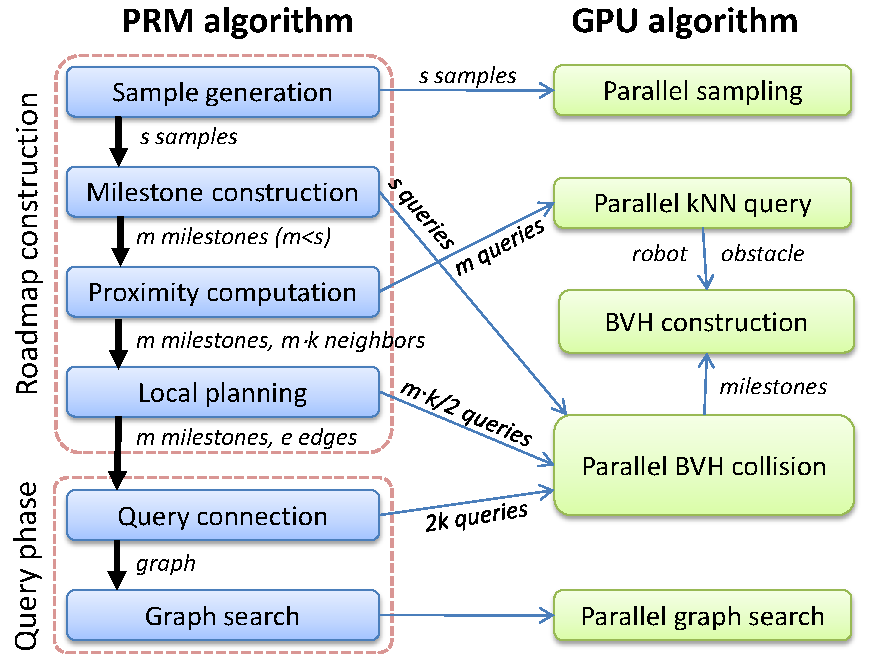
\includegraphics[width=0.9\linewidth]{figs/4/algorithm_overview.pdf}
  \caption[An overview of serial PRM and the GPU-based planner]{PRM overview and parallel components in our algorithm}
  \label{fig:4:GPU}
\end{figure}


\section{Parallelized PRM Motion Planning Algorithm}
\label{sec:4:algorithm}
In this section, we provide details about our algorithm and describe how each step is parallelized.

\subsection{Hierarchy Computation}
We construct a bounding volume hierarchy (BVH) for the robot and one for each of the obstacles in the environment, to accelerate the collision queries. We use the GPU-based construction algorithm introduced in~\cite{LauterbachGSLM09}, which can construct the hierarchy of \emph{axis-aligned bounding boxes} (AABB) or \emph{oriented bounding boxes} (OBB) in parallel on the GPU, for given triangle representation. For collision detection, we use the OBB hierarchy as it provides higher culling
efficiency and improved performance on GPU-like architectures. These hierarchies are stored in the GPU memory and we apply appropriate transformations for different configurations.

\subsection{Roadmap Construction}
The roadmap construction phase tries to capture the connectivity of the free configuration space, which is the main computationally intensive part of the PRM algorithm.

\subsubsection{Sample Generation}
We first need to generate random samples within the configuration space. Since samples are independent, we schedule enough parallel threads to utilize the GPU and use MD5 cryptographic hash function~\cite{Tzeng08} which in practice provides good randomness without a shared seed.

\subsubsection{Milestone Computation}
For each configuration generated in the previous step, we need to check whether it is a milestone: i.e., a configuration that lies in the free space and does not collide with obstacles. We use a hierarchical collision detection approach using BVHs to test for overlap between the obstacles and the robot in the configuration defined by the sample. The collision detection is performed in each thread by using a traversal algorithm in the two BVHs. The traversal algorithm starts with the two BVH root nodes and tests the OBB nodes for overlap in a recursive manner. If two nodes overlap, then all possible pairings of their children should be recursively tested for intersection.

We also use GPUs to compute the actual BVH structure for both the robot and obstacles by using a parallel hierarchy construction algorithm~\cite{LauterbachGSLM09}. Since the robot's geometric objects move depending on the configuration, its BVH is only valid for the initial configuration. In order to avoid recomputing a BVH for each configuration, we instead transform each node of the robot's BVH with the current configuration sample before performing overlap tests. Thus, only nodes that are actually needed during collision testing are transformed.

Previous work~\cite{Lauterbach10} has used BVH collision on GPUs to parallelize the tests within one query. The approach here is different because we instead parallelize a high number of collision queries, so each thread checks a fully independent collision. In addition, we do not need to find the actual intersection, just whether one exists or not. Thus, we can abort the traversal operation as soon as any collision is found and do not have to exhaustively search the hierarchy. In our implementation, each thread performs traversal in a stack-based depth first search (DFS) algorithm. We can store the DFS stack in the shared memory of the GPU, which has a higher access speed than the global memory on the GPU. Moreover, the DFS algorithm supports early exit from the traversal when the first collision between leaf nodes is computed.

\subsubsection{Proximity Computation}
For each milestone computed, we need to find its $k$-nearest neighbors. In general, there are two types of $\knn$ algorithms: exact $\knn$ and approximate $\knn$, which is faster by allowing a small relaxation.
Unlike previously proposed GPU solutions using brute force~\cite{Garcia08}, our proximity algorithm is based on a range query that uses a BVH structure of the points in configuration space. We describe the method for 3-DOF robots and then present its extension for high-DOF robots.

For $3$-DOF Euclidean space, we first construct the BVH structure for all the milestones using a parallel algorithm~\cite{LauterbachGSLM09}. For each configuration $\mathbf{q}$, we enclose it within an axis-aligned $\epsilon$ box: a box with $\mathbf{q}$ as the center and with $2\epsilon$ as the edge length. Next, we traverse the BVH tree to find all leaf nodes (i.e., configurations) that are within the $\epsilon$ box. This reduces to a range-query for $\mathbf{q}$. For a non-Euclidean DOF, we duplicate samples to transform it into a Euclidean space locally. For example, suppose one DOF is the rotation angle $\alpha \in [0, 2\pi]$. We add another sample $\alpha^* \in [-\pi, 3\pi]$ with a distance $2\pi$ to $\alpha$. If all 3-DOF are rotations, we need to add another $7$ samples for each milestone. Once the range query finishes, we choose the $k$-nearest ones from all the query results; this gives us the exact nearest neighbors.

For high dimensional spaces, we use a decomposition strategy to compute the approximate nearest neighbors. We use $6$-DOF as an example. We first decompose each configuration $\mathbf{q}$ into $3$-DOF projections $\mathbf{q_1}$, $\mathbf{q_2}$ and obtain two $3$-DOF groups. For each of them we build separate BVHs and perform range queries. Suppose we find $k_1$ neighbors within $\mathbf{q_1}$'s $\epsilon_1$ box and $k_2$  neighbors within $\mathbf q_2$'s $\epsilon_2$ box. We then compute the distances of these candidates to $q$ in $6$-DOF space and choose the $k$ of them that are nearest to $q$. For configuration spaces with higher dimensions, we just repeat the above process until all dimensions are considered. The final result is the approximate $\knn$ that has a distance to $\mathbf{q}$ of at most $\sqrt{3}\sum_i \epsilon_i$.

To further improve the performance of proximity computation in high dimensional space, we have developed a new $k$-nearest neighbor algorithm, which uses locality sensitive hashing (LSH) and cuckoo hashing to efficiently compute
approximate $k$-nearest neighbors in parallel on the GPU.

\subsubsection{Local Planning}
Local planning checks whether there is a local path between two milestones, which corresponds to an edge on the roadmap. Many methods are available for local planning. The most common way is to discretize the path between the two milestones into $n_i$ steps; we claim the local path exists when all the intermediate samples are collision-free, determined by performing discrete collision queries (DCD) at those steps. We can also perform local planning by using continuous collision detection (CCD), a local RRT algorithm or computing distance bounds~\cite{Schwarzer05}.

Local planning is the most expensive part of the PRM algorithm. Suppose we have $n_m$ milestones, and each milestone has at most $n_k$ nearest neighbors. Then the algorithm performs local planning at most $n_m \cdot n_k$ times. If we use DCD, then we need to perform at most $n_l = n_m \cdot n_k \cdot n_i$ collision queries, which can be very high for a complex benchmark.
For multi-query problems, this cost can be amortized over multiple queries as the roadmap is constructed only once. For a single-query problem, computing the whole roadmap is too expensive.

Therefore, in the single-query case, we use a lazy strategy to defer local planning until absolutely necessary.
Given a query, we compute several different candidate paths in the roadmap graph from the initial to final configuration and only check local planning for roadmap edges on the candidate paths. Local planning may conclude that some of these edges are not valid, and in that case, we delete them from the roadmap. If there exists one candidate path without invalid edges, the algorithm has found a collision-free solution. Otherwise, we compute candidate paths again on the updated roadmap and repeat the above process. This lazy strategy can greatly improve performance for single queries.

\subsection{Query Phase}
The query phase includes two parts: connecting queries to the roadmap and executing graph searches to find paths.
\subsubsection{Query Connection}
Given the initial-goal configurations in a single query, we connect them to the roadmap. For both of these configurations, we find the $k$ nearest milestones on the roadmap and add edges between the query and milestones that can be connected by local planning. We use the same algorithm from the roadmap construction phase, except that the $k$ used is $2-3$ times larger in order to increase the probability of finding a path.

\subsubsection{Graph Search}
The search algorithm tries to find a path on the roadmap connecting initial and goal configurations. Many solutions exist for this, such as DFS, BFS, A*, and R*~\cite{JK10-ICRA}. A* and R* can find the shortest path, which is not necessary for the basic motion planning problem. Moreover, A* and R* are not efficient when a lazy strategy is used. As a result, we use DFS or BFS. For the multi-query case, each GPU thread traverses the roadmap for one query using DFS and the final results are collision-free paths. For the single-query case, we exploit all the GPU threads to find the path for one query using a BFS search: for nodes that are the same number of steps away from the initial node, we add their unvisited neighbors into the queue in parallel. In other words, different GPU cores traverse different parts of the graph. The main challenge of this method is that work is generated dynamically as BFS traverse progresses, and the computational load on different cores can change significantly. To address the problem of load balancing and work distribution so that parallelism for all cores is maintained, we use the light-weight load balancing strategy in~\cite{Lauterbach10}.

Since BFS is time-consuming, we use lazy strategy to further improve the graph search's performance. When using a lazy strategy, we first run BFS for several iterations to find a set of nodes that are reachable from initial node. Then we run DFS/BFS/A* in each thread with one of these nodes as the initial node and find several candidate paths. We use local planning to check whether any one of these are collision-free paths. If yes, we return a valid path. Otherwise, we remove all invalid edges from the roadmap and repeat the process again.


\section{Implementation and Results}
\label{sec:4:result}
In this section, we present details of our implementation and evaluate the performance of our algorithm on a set of benchmarks. All the timings reported here were taken on a machine using a Intel Core i7 CPU ($\sim$\$600) at 3.2GHz CPU and 6GB memory. We implemented our algorithms using CUDA on a NVIDIA GTX 285 GPU ($\sim$\$380) with 1GB of video memory.

Our algorithm is designed to work well on any massively processor- and data-parallel architecture by using vector parallelism and low synchronization overhead. In this regard, both NVIDIA and ATI (as well as Intel's Larrabee processor) are relatively similar. We used CUDA since it was the most stable development platform at the moment, but look forward to testing in OpenCL and comparing across architectures.

\begin{figure}[htb]
  \centering
  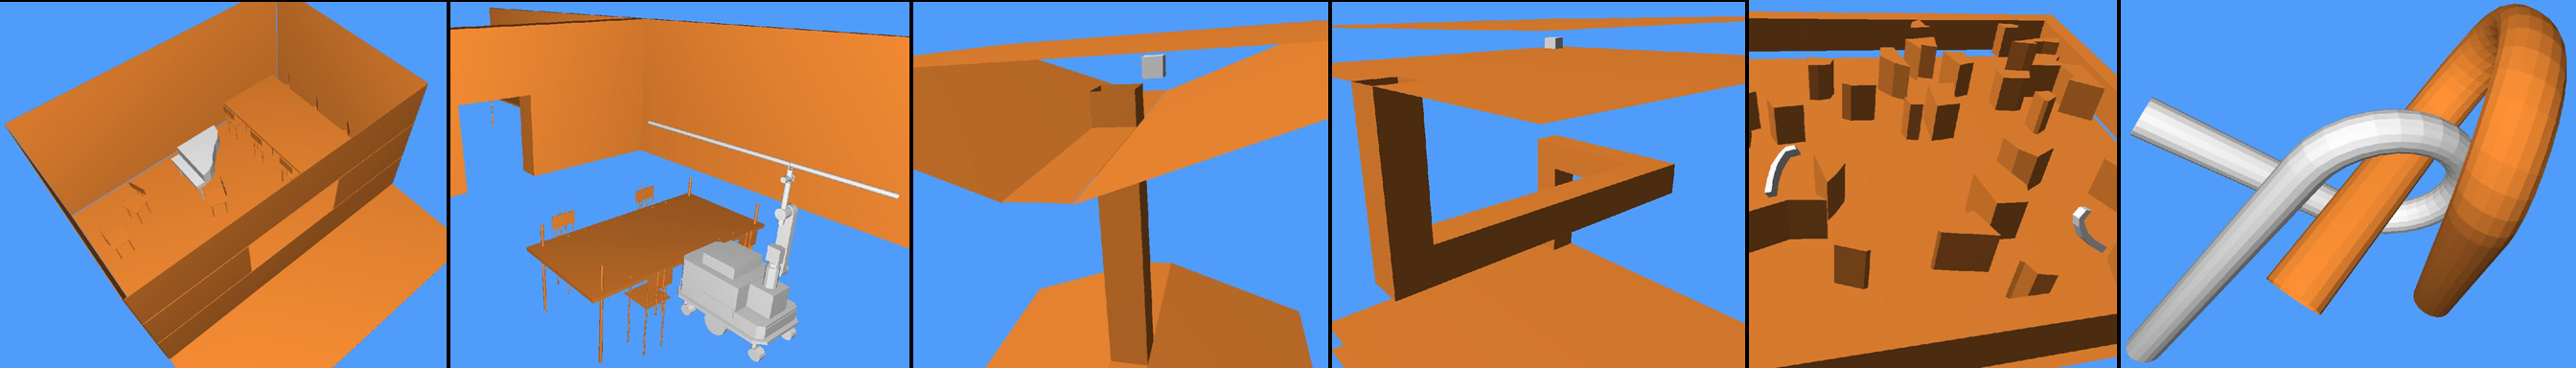
\includegraphics[width=0.9\linewidth]{figs/4/benchmarks.png}
  \caption[Benchmark scenes used for the GPU-based planner]{The benchmark scenes used for our algorithms in the following order: piano (2484 triangles), helicopter (2484 triangles), maze3d1 (40 triangles), maze3d2 (40 triangles), maze3d3 (970 triangles), and alpha puzzle (2016 triangles).}
  \label{fig:4:benchmarks}
\end{figure}

We implement the PRM algorithm on the GPU (G-PRM) for multi-query planning problems and implement its lazy version (GL-PRM) for single-query problems. We compare these with the PRM and RRT algorithms implemented in the OOPSMP library~\cite{plaku+2007:OOPSM}, which is a popular library for motion planning algorithms on CPU. The benchmarks used are shown in Figure~\ref{fig:4:benchmarks}. Our comparisons are designed as follows: for each benchmark, we find a suitable setting where C-PRM finds a solution, and then we run G-PRM with a comparable number of samples. After that we run GL-PRM with the same setting as G-PRM, and run C-RRT with the same setting as C-PRM. Of course, the compared PRM algorithms on GPU and CPU are not identical in terms of the final result, for instance, due to underlying random sample generation. Even though these random generators are slightly different, the number of collision-free nodes and collision-free arcs in the computed roadmaps are comparable. Moreover, the final paths computed by GPU algorithms are close to those computed by CPU algorithms. In practice, the total work performed by the non-lazy GPU planner is actually higher than the CPU version.

Table~\ref{tab:4:complexity} shows the comparison of timings between algorithms. In general, G-PRM is about 10 times faster than C-PRM, and GL-PRM can provide another 10-fold acceleration for single query problems. G-PRM is faster than C-PRM even for dynamic scenes. The current C-RRT and C-PRM are both single-core versions. However, even a multi-core version of PRM would only improve the timing by 4-fold at most, because on a 8-core CPU it is hard to scale the hierarchy computations and nearest neighbor computations linearly. Therefore, our GPU algorithms can still provide performance 1-2 orders of magnitude higher than CPU algorithms.

Figure~\ref{fig:4:breakdown} shows the timing breakdown between various steps for G-PRM and GL-PRM. The difference between the performance of two algorithms is clear: in G-PRM, local planning is the bottleneck and dominates the timing, while in GL-PRM graph search takes longer because local planning is performed in a lazy or output-sensitive manner. In GL-PRM, three components take most timing: milestone construction, proximity computation, and graph search, because all of them may perform collision queries heavily. If the environment is cluttered and the model has complex geometry, milestone construction will be slow (\emph{Alpha puzzle} in Fig~\ref{fig:4:breakdown}). If the environment is an open space and has many milestones, proximity computation will be the bottleneck (\emph{mazed3d2} in Fig~\ref{fig:4:breakdown}). If the lazy strategy can not guess a correct path, then graph search will be computationally intensive due to the large number of collision queries (\emph{maze3d3} in Fig~\ref{fig:4:breakdown}). However, in all these environments, GL-RPM all outperforms other methods.

We test the scalability of G-PRM and GL-PRM on the \emph{maze3d3} benchmark and the result is shown in Fig~\ref{fig:4:scalability}. It is obvious that GL-PRM is generally faster than G-PRM, and both algorithms achieve near-linear scaling on the benchmark. However, observe that as the number of samples increases, GL-PRM slows down faster than G-PRM. This is because when the number of samples increases, proximity computation becomes increasingly expensive and dominates the timing when the number of samples is near $1$ million.

\begin{table}[htb]
\begin{center}
\begin{small}
\begin{tabular}{|c|c|c|c|c|c|} \hline
               & C-PRM & C-RRT & G-PRM & GL-PRM \\ \hline \hline
piano          & 6.53s   &  19.44s &   1.71s   &     111.23ms      \\  \hline
helicopter          & 8.20s     &  20.94s    &  2.22s    &  129.33ms      \\ \hline
maze3d1        & 138s  &  21.18s    &     14.78s &     71.24ms    \\ \hline
maze3d2        & 69.76s &  17.4s   &   14.47s   &      408.6ms   \\ \hline
maze3d3        & 8.45s   &   4.3s   &  1.40s    &     96.37ms    \\ \hline
alpha1.5       & 65.73s  &   2.8s   &    12.86s  &   1.446s      \\ \hline
\end{tabular}
\end{small}
\end{center}
\caption[Performance comparison between the PRM and RRT implementations in OOPSMP and the GPU-based planner]{The left two columns evaluate the performance of the PRM and RRT algorithms in the OOPSMP. The right two columns evaluate the performance of our GPU-based algorithms.}\label{tab:4:complexity}
\end{table}

\begin{figure}[htb]
  \centering
  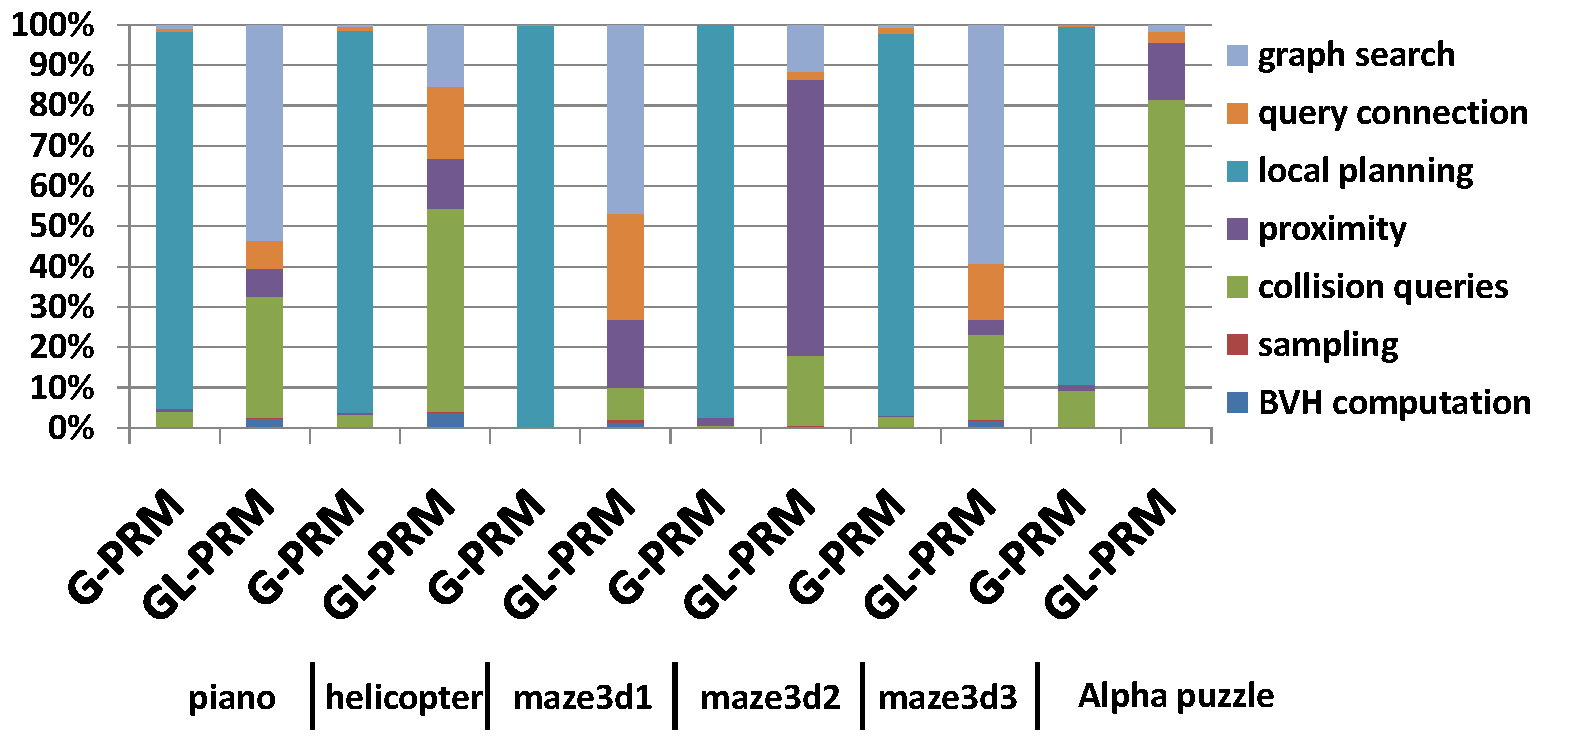
\includegraphics[width=0.9\linewidth]{figs/4/breakdown.pdf}
  \caption[Split-up of timings for the GPU-based planner]{Split-up of timings: the fraction of time spent in different parts of the G-PRM and GL-PRM.}
  \label{fig:4:breakdown}

  \centering
  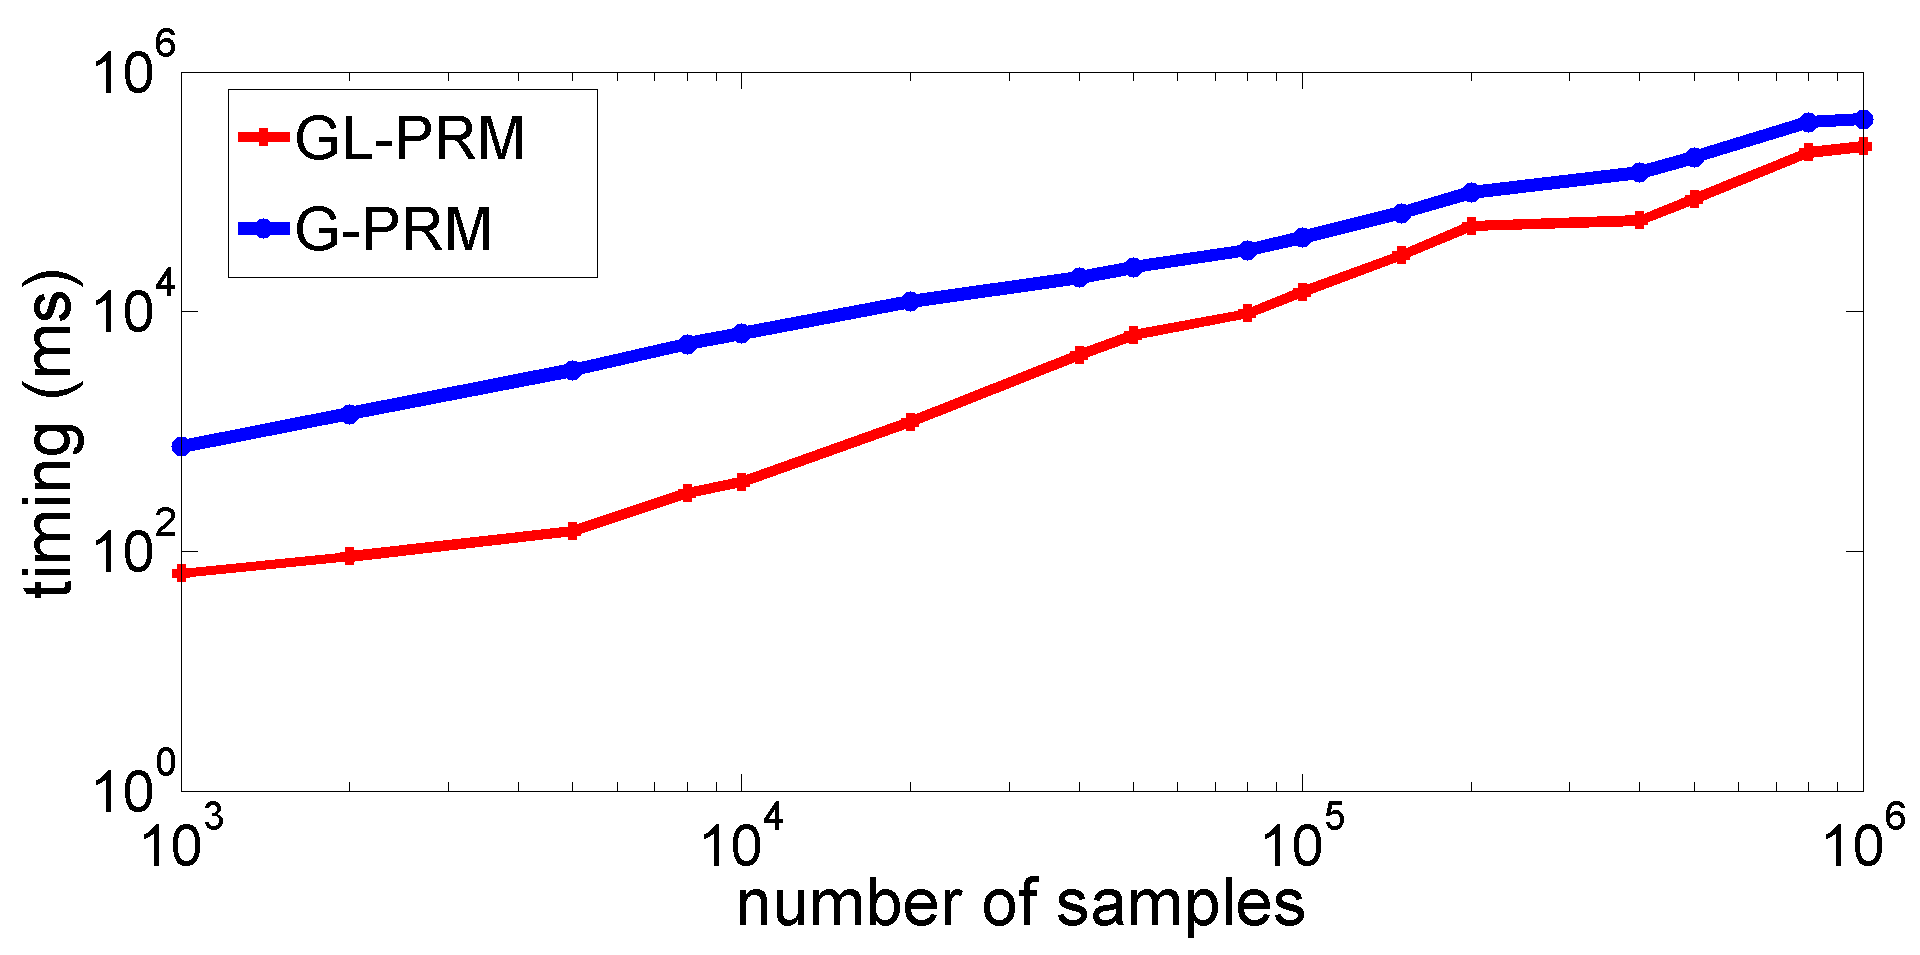
\includegraphics[width=0.9\linewidth]{figs/4/scalability.png}
  \caption[The scalability of G-PRM and GL-PRM algorithms]{The scalability of the G-PRM and GL-PRM.}
  \label{fig:4:scalability}
\end{figure}

\section{Conclusions and Future Work}
In this chapter, we have introduced a complete motion planning algorithm on GPUs. Our algorithm can exploit all the parallelism within the PRM algorithm, including the high-level parallelism provided by the PRM framework and the low-level parallelism within different components of the PRM algorithm, such as collision detection and graph search. As a result, our method provides performance 1-2 orders of magnitude higher than previous CPU-based planners. This makes our method the first to perform real-time motion planning and global navigation in general environments.
There are many avenues for future work. For instance, we are interested in extending the GPU planning algorithms to high-DOF articulated models. We are also interested in using exact algorithms for local planning. Moreover, we hope to apply our real-time algorithms to dynamic scenarios. Lastly, we will test our algorithm in OpenCL/DirectX11 and compare across different architectures.
